\chapter{Agent Based Modeling and Simulation}
\label{Chapter.three}

Interdependencies in the systems are getting complex day by day, and therefore we need more precise modeling methodologies. Modeling complex systems can be done using agents. Modeling a system with agents is named as Agent Based Modeling (ABM). Using ABM, it is possible to simulate the functionality of large scale models involving autonomous agents, in order to evaluate the performance of the system as a whole. ABM also allows us to visualize the results of simulation in a graphical manner. These results are generally utilized to evaluate and draw conclusions from the behavior of the system, which in turn validates the ABM's specification~\cite{Barbosa2011}. 

\vspace{3mm}
Agent based approach has the following characteristics~\cite{christian06}:

\begin{enumerate}
\item It is capable of providing a natural environment for study of huge complex systems.
\item While developing geospatial models, agent based approach is more flexible when compared to other approaches.
\item Capable of capturing the transient behavior of system.
\end{enumerate}

\vspace{5mm}

An agent based model comprises of three major elements. They are agents, relationships among agents and methods for their interaction, and the environment under which agents operate~\cite{macal2010}. Detailed explanation to these elements can be found in section~\ref{section.Agent}. The task of the model developer is to analyze and decide on the number of needed agents, the required relationships between agents and the type of environment to create that particular agent based model. The developer should be able to model, identify and program the above elements. To run a model, there is a need for a computational engine in order to simulate the agent's behaviors and their respective relationships.

\section{Multi Agent Systems}

ABM has become a more powerful approach in many fields. It provides an efficient way to model complex systems using agents whose behavior can be different from one another. These kind of systems where there are multiple agents which interact and act autonomously are called Multi Agent Systems (MAS). MAS~\cite{peer} is a collection of unrelated and dissimilar interacting agents. As it is not possible for a single agent to handle several complex tasks, there is a need for using multiple individual agents in a single system. These agents interact with each other in order to resolve the existing obstacles. The ability of an agent can be analyzed by the collaboration~\cite{Dunin2010} it does with other agents to solve a particular problem when encountered. At the time of designing a multiagent system, we need to consider the behaviors of all the agents in the environment. Agents in the multiagent systems need not be application specific. They can also be generic agents with their own behaviors. 

Before designing an agent based model, the model developer should create a design specification of what he/she needs to implement. This design specification should include the following information about the model. 

\vspace{3mm}
\begin{enumerate}
\item How many agents should the model contain?  
\item What are the responsibilities of each individual agent? 
\item How they should interact with the environment and fellow agents?
\item What kind of data an agent needs and from where it should retrieve the data from?
\item What kind of environment that model should contain? 
\item What kind of data an environment needs to have about an agent? 
\item What are the other individual components this model should contain?
\end{enumerate}

\vspace{5mm}

This is the essential information which we should know before designing a model. Once the specification is created, environment, individual components and agents should be created according to the specification. Once the agent based model is created, it should be simulated using agent based modeling toolkits which are described in more detail in Section~\ref{section.Sim}.
 
Agent Based Modeling and Simulation (ABMS) has roots in the field of MAS, robotics, Artificial Intelligence (AI), game theory, computational sociology and evolutionary programming. ABMS can be defined as a set of techniques, rules and tools for implementing computation models for complex adaptive systems~\cite{macal2010}. It comprises of many interactive components and also agents which are capable of doing complex adaptive tasks. ABM tools provide a good support when designing a system model by using MAS system. There is a need for Agent based modeling toolkits in order to run an agent based model. Running an agent based model means, to have all the components and simulating agents which execute their interactions and behaviors in the environment. 

\section{Agent}
\label{section.Agent}

It is worthless to build a system without knowing how it reacts in complex situations. We should test the functionality before building any complex systems. Agents can be used to test the functionality of a system. An Agent is described as an independent component which is capable of making intelligent decisions to complex situations~\cite{Bonabeau2001}. Agents are usually more active rather than being passive~\cite{macal2006}. Each agent has its own set of attributes and methods as illustrated in Fig.\ref{fig:3.1}. Method of an agent defines its behavior. Each agent has its own behavior. Agents attributes can be both static and dynamic. Static attributes cannot be changed, whereas dynamic attributes can be changed during the simulation. An agent can communicate with another agent and to its environment. Agents are capable of learning from the environment. Some of the features of an agent are discussed below:

\begin{figure}[H]
\vspace{12mm}
\centering
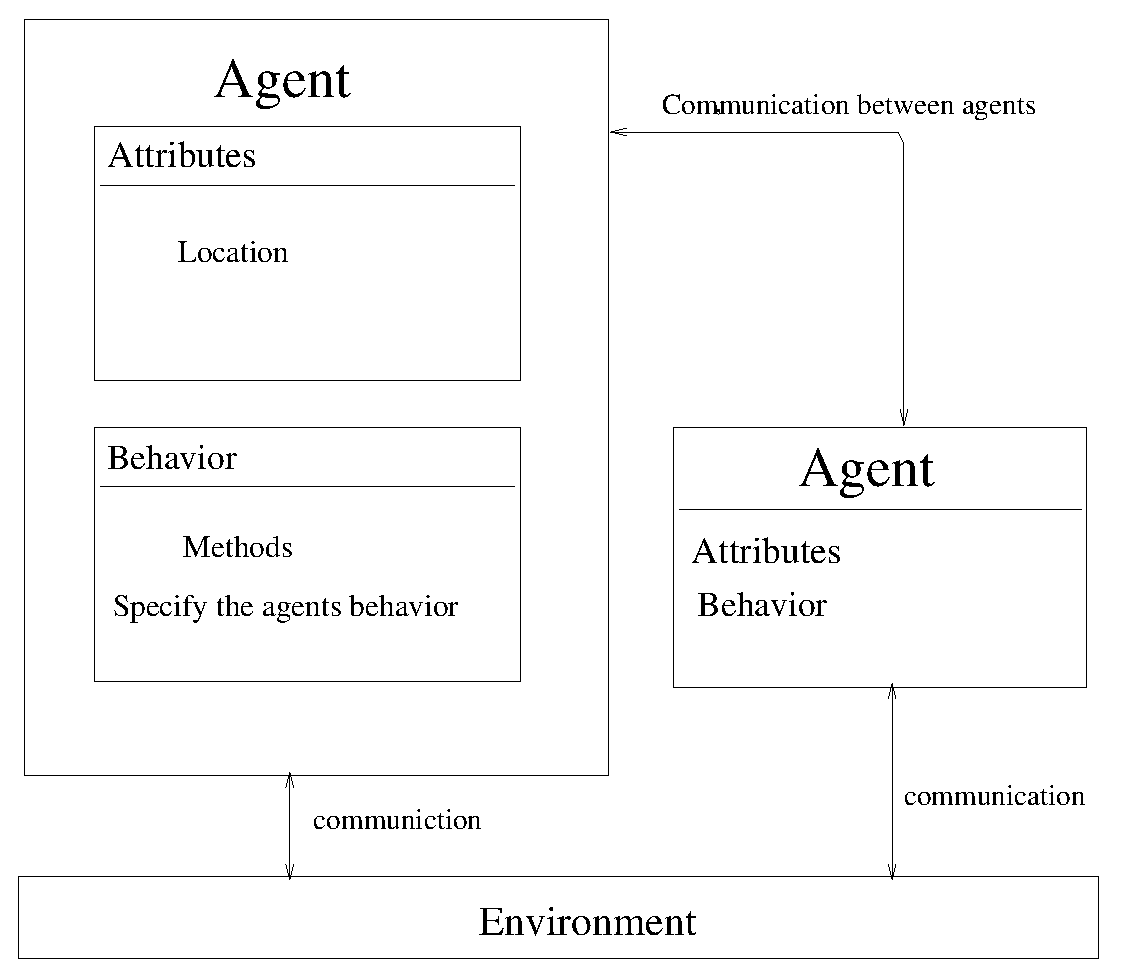
\includegraphics[height=4.8in, width=5.1in]{agent.eps}
\caption{Agents interaction with environment.}
\label{fig:3.1}
\vspace{10mm}
\end{figure} 

\vspace{0.5cm}
\noindent\textbf{Autonomous}
\vspace{5mm}

\noindent While simulating a model, agents can act according to their own decision without any external interference. Agents act autonomously and perform spontaneous actions according to the changing situations. 

\vspace{0.5cm}
\noindent\textbf{Goal Oriented}
\vspace{5mm}

\noindent An agent can be goal oriented. It can be designed to follow a specific algorithm in order to accomplish certain goals.

\vspace{0.5cm}
\noindent\textbf{Reusable}
\vspace{5mm}

\noindent Agents are designed to be reusable. An agent once created can also be used in any other environment.

\vspace{0.5cm}
\noindent\textbf{Interactive}
\vspace{5mm}

\noindent Agents can communicate with other agents and also can interact with the environment. Environment is the medium where agents and other components of the model are present. By exchanging data with environment an agent can know the state of other components existing in the same environment. There is a possibility to have several agents in an environment, in this case each agent has its own behavior. The environment in which the agents act may not be reliable. 

For instance, consider an environment which has some paths, intersections and an agent that moves along the paths. Here an agent should have the knowledge of paths and intersections and should be able to navigate among them. This can only be possible if the agent can access the required information from the environment. The agent should be capable of taking independent decision to know whether it is in the correct path or not. When the agent is at intersection of two paths the agent should choose one of the paths based on the predefined instructions. We design the agent in such a way that it will be able to take the decision and act accordingly in all the cases. If we design the agent to take a random path at intersections, then the agent will do so whenever it encounters an intersection. It is also possible to design an agent with complex behavior which can handle complicated tasks. This is how the agents fulfill the interactive property.

\vspace{10mm}
\noindent\textbf{Self Directive}
\vspace{5mm}

\noindent In some situations there is a need for two agents to communicate with each other. For example, if there is a moving and stable agent in the environment, the moving agent should detect the stable agent when they are close to each other, and vice versa. Sometimes, the agents may need one another's coordinates in order to identify each other. This task will be accomplished only if both the agents can communicate with each other and share data among them such as coordinates and state of the agent. An agent can be self directive, as in this case the moving agent directs itself based on the information it retrieves from the environment.

\vspace{3mm}
Apart from the above mentioned properties, there are few more characteristics of agents which are stated below:

\begin{enumerate} 
\item Agents are capable of interacting and influencing other agents while having independent behavior.
\item Agents are adaptive to their environments, which means that agents must be designed to function properly even in unpredictable environments. 
\item Agents should be trained to accomplish a particular task regardless of the given environment. If we train agents in this way, it will be possible to reuse the same agent in different environments for similar functionality.
\item Agents can be heterogeneous; meaning that each agent can have its own property and behavior and therefore we cannot expect two communicating agents to be behaving in the same way.
\end{enumerate} 

\vspace{5mm}

\begin{figure}[H]
\vspace{5mm}
\centering
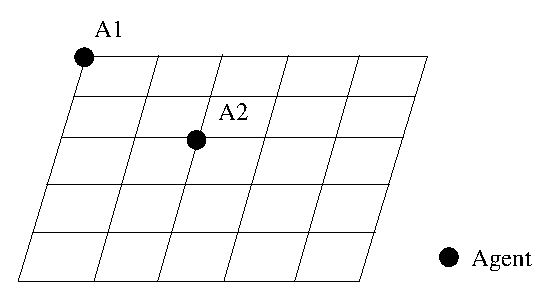
\includegraphics[height=2.9in, width=3.5in]{noc.eps}
\caption{Agents and environment.}
\label{fig:3.2}
\vspace{10mm}
\end{figure}

Figure.\ref{fig:3.2} illustrates the grid environment. Where A1 and A2 are moving and stable agents, respectively. A1 and A2 can interact with the grid directly. Both agents have different methods which specify their behaviors. A1 chooses a random path when it comes across an intersection, whereas A2 is stable at particular location. A1 moves along the grid and randomly changes its direction at each node, A2 should take a note whether or not A1 has passed by. In this particular case, A1 should know whether it has arrived at A2's location, which means that A1 should interact with environment and check whether A2 is present at current position or not. Here A2 should also have the information about A1 to determine whether A1 is passing through it or not. This can be achieved only if we design the agents in such a way that they interact with each other when necessary. The above example illustrates the adaptability property of agents. This model comes under multiagent systems because agents in this model have different properties and behaviors. 

\section{Simulation Environments}
\label{section.Sim}

There are many simulation environments~\cite{rob} which can be used for multiagent simulations. Simulation environments can also be called as simulators. We will specify them as simulators throughout this section for convenience. Simulators are categorized into three main types. They are behavior based simulators, compiled multiagent simulators and interpreted multiagent simulators. 

\subsection{Behavior Based Simulators}

Teambots~\cite{Balch2000} simulator belongs to this category. It is a light weight Java based robotics simulation environment. Teambots provides graphical display, minimal robot and physical sensor facilities and a simple schedule procedure. It is mostly used for behavior based robotic applications. This simulator has the distinction between the agents which drive the objects (robotic software) and objects in the world (robots). Teambots can port the robotic agent behaviors to the real robots with the help of real-robot application protocol interfaces (APIs).

In research paper~\cite{MASON2005}, it was presented that implementing non-robotic multiagent simulations with an existing Teambots simulator involved modifying and adding significant amount of new functionality. This has added serious overhead to their codebase which slowed their experiment and has introduced many bugs. Owing to this limitation, it cannot be used for all kinds of applications.


\subsection{Compiled Multiagent Simulators}

There are several Compiled multiagent simulators, for example, SWARM~\cite{Paul2000}, RePast~\cite{Repast2001, Repast}, Ascape~\cite{Miles2001, Ascape} and  Multi-Agent Simulator of Neighborhoods (MASON)~\cite{MASON, MASON2005, MASONMANUAL2011}. 

The earlier version's of SWARM applications have been written in Objective-C and Tcl/Tk in order to schedule. It can now run the applications written in Java which uses special libraries to communicate with Objective-C. The usage of unusual language in the simulator has become a challenging endeavor for the developers to further extend and maintain SWARM.

After analyzing the complications in SWARM simulator, RePast has envisioned to re-implement most of SWARM's ideas either in Java or .NET. In recent years, it has become a greatly used multiagent simulator. RePast distribution is now widely used for modeling applications such as neural networks, GIS, charts, graphs and social network modeling.

On the other hand, an Ascape multiagent simulator is a rule oriented framework written entirely in Java. Agents in these applications have specific rule based behaviors and they are scheduled according to certain environmental conditions. These agents are grouped in huge structures which are then scheduled in an order specified by user (and/or scheduler). This framework is efficient and only suitable for model development in few cases. It also imposes constraints on the whole schedule, particularity in cases where there is a need for arbitrary agent handling.

MASON simulator provides graphical visualization, event monitoring, generation of various forms of media and event ordering. These functionalities can also be provided by the above discussed three multiagent simulators. Apart from these similarities, MASON also have some major differences: MASON provides 3D fields, both 2D and 3D field visualizations in 3D and more efficient and flexible 2D visualization. MASON is faster in visualizing models when compared to other simulator toolkits. MASON is also capable of providing duplicable results when necessary, where as most of the simulators are not. MASON models can be separated from visualization dynamically. The above mentioned frameworks run ``headless'' (i.e. a model can run without visualization) and it is not possible to migrate a headless process to another machine during mid-run. Visualization is much less in headless processes. Generally, many simulators are designed for creating single-shot models. That is, in these kind of models, a developer will construct and run a model once and then analyze the results. In MASON, it is possible to run the models as many times as possible without any complications. The models can also be check-pointed and migrated to other machines, and it is possible to get the duplicable results.


\subsection{Interpreted Multiagent Simulators}

In Interpreted Multiagent Simulators, a user can manipulate the existing world by using interpreted programming language such as Logo. Instead of making minor changes to the model before compile time, a user can directly modify the code at runtime to examine the effects. This eliminates several compile and run cycles for the entire model. This is design strategy behind StarLogo~\cite{Mitchel, StarLogo} and NetLogo~\cite{Uri}. These simulators have same basic functionality like in SWARM. Unlike in SWARM, the language used by developers to implement the model in these simulators is a modified version of Logo. Breve~\cite{Jon, Breve} is also a similar simulator which can handle 2D and 3D worlds with which the user can manipulate control objects with the help of ODE physics engine and a proprietary language named as Steve. These simulators have many benefits such as instant feedback on change of code and encourages mid-run. The benefits of Breve are: it wraps the powerful physics 
environment with easy to learn library. According to the theory, it is observed that interpreted language model can dynamically add and remove visualization and can be ported easily in mid run between any two platforms. The main disadvantage of these simulators is that it can be slower for complex models. The schedules built with these simulators are mainly constrained by their respective graphical interfaces. Rapidly building models using this language make them an attractive proposition for model developers. But, at the same time this would lead to long runtimes for complex simulations. 

Considering all the above simulators and their pros and cons, we have come to the conclusion that we will use MASON (agent based modeling toolkit) for this thesis to model and simulate a Network-on-chip. In Chap.~\ref{Chapter.four}, we will give an overview on MASON and its architectural design. 
